\documentclass{article}



\usepackage{arxiv}

\usepackage[utf8]{inputenc} % allow utf-8 input
\usepackage[T1]{fontenc}    % use 8-bit T1 fonts
\usepackage{hyperref}       % hyperlinks
\usepackage{url}            % simple URL typesetting
\usepackage{booktabs}       % professional-quality tables
\usepackage{amsfonts}       % blackboard math symbols
\usepackage{nicefrac}       % compact symbols for 1/2, etc.
\usepackage{microtype}      % microtypography
\usepackage{lipsum}		% Can be removed after putting your text content
\usepackage{graphicx}
\usepackage{amsmath}
\usepackage{witharrows} % Equation arrows
\usepackage{cleveref} % Better equation management
\usepackage{doi}
\usepackage{float}
\usepackage{subcaption}
\usepackage{dirtytalk}

% Tikz for graphics and graph drawing
\usepackage{tikz}
\usetikzlibrary{graphs, graphdrawing, graphs.standard, quotes, decorations.pathmorphing, arrows.meta, matrix,decorations.pathreplacing}
\usepackage{listofitems} % For the NN figures
\usepackage[outline]{contour} % glow around text
\contourlength{1.4pt}

\usegdlibrary {force}

% Plots
\usepackage{pgfplots}

\usepackage[backend=biber, style=authoryear, citestyle=authoryear, maxcitenames=2, mincitenames=1, uniquename=false]{biblatex}
\addbibresource{references.bib}
\let\cite\autocite
\crefname{figure}{Figure}{Figures}
\crefname{table}{Table}{Tables}

% Advanced glossary and acronym management
\usepackage[acronym, automake]{glossaries-extra}
\setabbreviationstyle[acronym]{long-short}
\loadglsentries{Acronyms}
\makeglossaries


\title{AmesFormer: A Graph Transformer Neural Network for Mutagenicity Prediction}

%\date{September 9, 1985}	% Here you can change the date presented in the paper title
%\date{} 					% Or removing it

\author{ \href{https://orcid.org/0000-0000-0000-0000}{\includegraphics[scale=0.06]{orcid.pdf}\hspace{1mm}Luke A.~Thompson}\thanks{Use footnote for providing further
		information about author (webpage, alternative
		address)---\emph{not} for acknowledging funding agencies.} \\
	School of Pharmacy\\
	The University of Sydney\\
	Sydney, Australia \\
	\texttt{Placeholder@Nothing.com} \\
	%% examples of more authors
	\And
	\href{https://orcid.org/0000-0000-0000-0000}{\includegraphics[scale=0.06]{orcid.pdf}\hspace{1mm}Josiah ?.~Evans} \\
	Independent Researcher\\
	% Mount-Sheikh University\\
	Seoul, Republic of Korea \\
	\texttt{Placeholder@Nothing.com} \\
    \And
	\href{https://orcid.org/0000-0000-0000-0000}{\includegraphics[scale=0.06]{orcid.pdf}\hspace{1mm}Slade T.~Matthews} \\
	School of Pharmacy\\
	The University of Sydney\\
	Sydney, Australia \\
	\texttt{Placeholder@Nothing.com} \\
	%% \AND
	%% Coauthor \\
	%% Affiliation \\
	%% Address \\
	%% \texttt{email} \\
	%% \And
	%% Coauthor \\
	%% Affiliation \\
	%% Address \\
	%% \texttt{email} \\
	%% \And
	%% Coauthor \\
	%% Affiliation \\
	%% Address \\
	%% \texttt{email} \\
}

% Uncomment to remove the date
%\date{}

% Uncomment to override  the `A preprint' in the header
%\renewcommand{\headeright}{Technical Report}
%\renewcommand{\undertitle}{Technical Report}
\renewcommand{\shorttitle}{AmesFormer}

%%% Add PDF metadata to help others organize their library
%%% Once the PDF is generated, you can check the metadata with
%%% $ pdfinfo template.pdf
\hypersetup{
pdftitle={AmesFormer},
pdfsubject={q-bio.NC, q-bio.QM},
pdfauthor={Luke A.~Thompson, Josiah ?.~Evans},
pdfkeywords={Ames, Mutagenicity, GNN, Transformer},
}

\begin{document}
\maketitle

\begin{abstract}
	The Ames mutagenicity test is a gold standard assay for the safety assessment of new chemicals. However, many \textit{in silico} models rely on challenging-to-interpret ensemble strategies and molecular fingerprint data which neglects gestalt molecular structure. To improve upon these models, we propose AmesFormer, a graph transformer neural network which shows state-of-the-art single model performance for the prediction of Ames mutagenicity. We briefly review the current state of Ames modelling with a focus on graph neural networks. We then discuss the architecture of AmesFormer with specific reference to the generalisation of transformer positional encodings to chemical data and efforts to make AmesFormer accessible to academic researchers. We benchmark AmesFormer using a standardised dataset against 22 other Ames models, achieving near-best-in-class performance. We then quantify the uncertainty of our performance metrics using a unique Bayesian approach. We support our findings with reference to other models from the literature and with theoretical developments in discrete mathematics and graph theory. Overall, we present a high-performance, accessible, and open-source computational model for Ames mutagenicity, with significant potential for regulatory and drug development applications. 
\end{abstract}


% keywords can be removed
\keywords{Ames \and Mutagenicity \and Neural Networks \and GNNs}


\section{Introduction}
\subsection{The Ames Assay}
The Ames test is a widely-used \textit{in vitro} mutagenicity assay essential to drug development. Ames data is explicitly required by many regulatory guidelines, such as \gls{ich} guideline S2 (R1) \cite{ich_ich_2013}. It thus represents a high bar to market access for pharmaceuticals, with many compounds rejected early in the case of an Ames-positive outcome \cite{honma_improvement_2019}.

In the Ames assay, a histidine-deficient substrate is inoculated with strain of auxotrophic mutant histidine-dependent Salmonella typhimirium \cite{ames_improved_1973}. This dependence is introduced via a mutation at the histidine operon \cite{ames_improved_1973}. A suspected mutagenic compound is then introduced. If the mutagen-containing substrate shows significantly greater colony growth than a control, the test-molecule has reversed the histidine-dependence mutation and is mutagenic. This simplicity has resulted in the Ames test having an excellent inter-laboratory replicability of 85\% \cite{kamber_comparison_2009}.

Different \textit{S. typhimurium} strains detect various mutagenicity mechanisms, which can be categorized into substitution mutations (SNPs) or frameshift mutations \cite{lui_mechanistic_2023}. The Ames test also includes S9 rodent liver homogenate, enabling the detection of mutagens that require metabolic activation \cite{maron_revised_1983, ames_improved_1973}.

\subsection{QSAR Modelling}
As the Ames test costs approximately \$2000 per chemical and the CAS reigstry grows by over 4000 molecules daily, the cost of \textit{in vitro} screening for every new chemical quickly becomes prohibitive \cite{honma_improvement_2019}.

To address this problem, \textit{in silico} \gls{qsar} models have been developed to provide cheaper and higher-throughput methods of Ames screening \cite{furuhama_evaluation_2023}. The use of such models is recommended within \gls{ich} guideline M7 (R1) for the control of mutagenic impurities in pharmaceuticals and the European Union's \gls{reach} agreement \cite{european_communities_regulation_2006, ich_assessment_2017, honma_improvement_2019}. \Gls{aicis} and \gls{fda} have also provided guidelines for implementing \textit{in silico} toxicity evaluation methods \cite{aicis_guide_2022, han_fda_2023}.

\subsection{Current Models}
The input to many Ames \gls{qsar} models are \glspl{mf}. \gls{mf}, as seen in \cref{fig:ndma_fp}, are vectorised binary representations of a molecule’s chemical features \cite{capecchi_one_2020}. 

\begin{figure}[H]
    \centering
    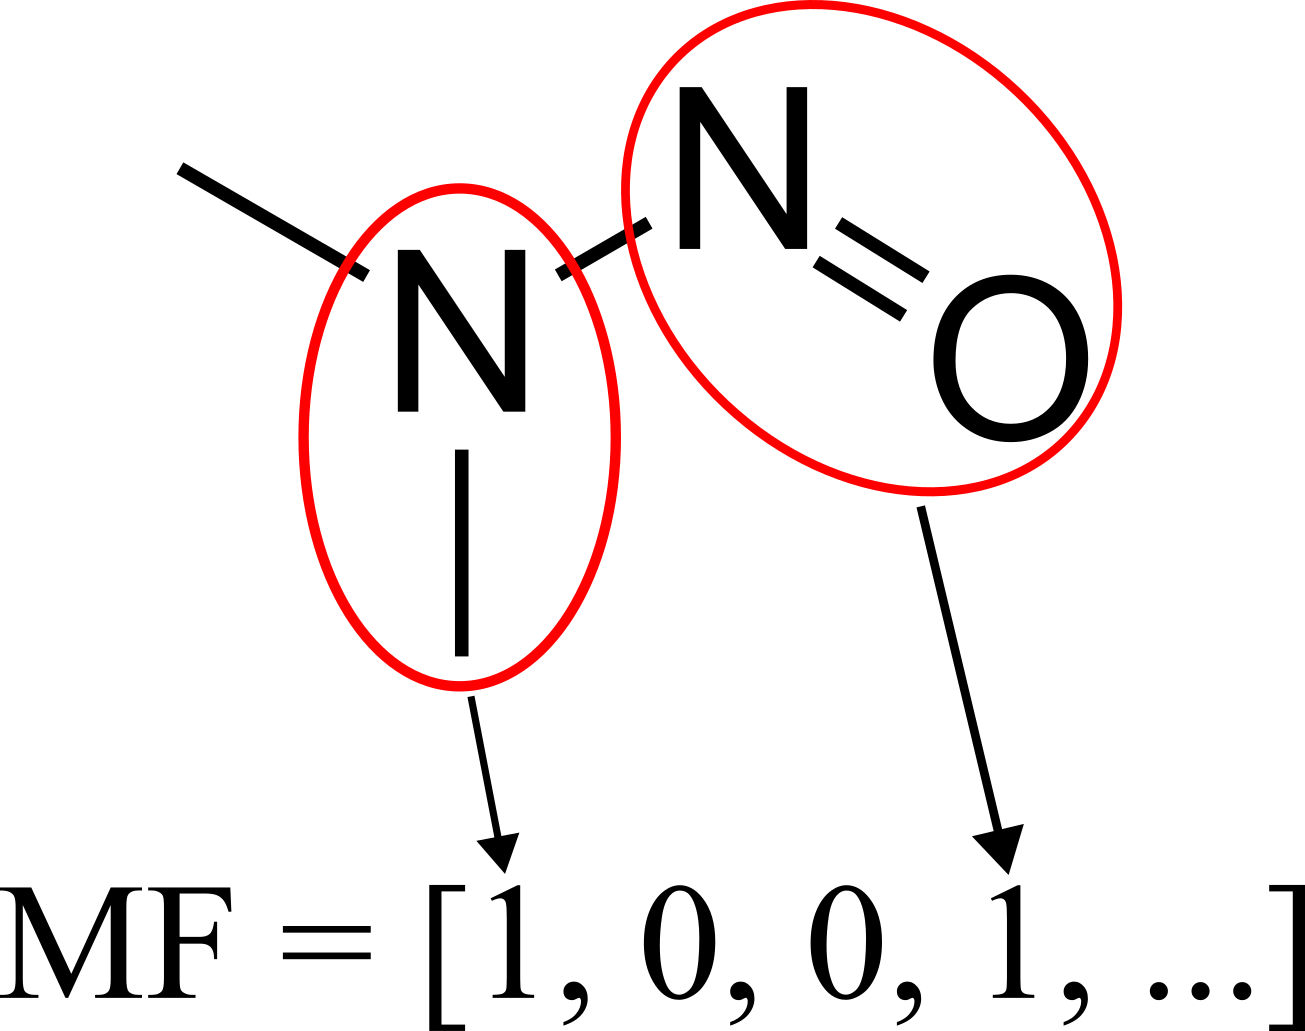
\includegraphics[width=0.35\linewidth]{Images/NDMA Fingerprint.png}
    \caption{An illustrative examples of the hashing of different \gls{ndma} substructrures into the \gls{mf} bit vector.}
    \label{fig:ndma_fp}
\end{figure}

Two fingerprinting methodologies are commonly applied to molecules within the Lipinski Limits. 
Structural key \glspl{mf}, such as \gls{maccs} keys seen in \cref{fig:maccs}, encode the presence of a set of predefined chemical substructures into a binary vector \cite{durant_reoptimization_2002, seo_development_2020}.
Hash \gls{mf} \textit{de novo} numerically encode non-predefined substructures. The archetypal \gls{morgan} \gls{mf} shown in \cref{fig:morgan} hashes the local environment (of arbitrary size) around each atom and encodes this into the bit vector representation \cite{rogers_extended-connectivity_2010}.

\begin{figure}[H]
    \centering
    \begin{subfigure}[t]{0.48\textwidth}
        \centering
        \begin{align*}
            \text{MACCS} &= \begin{bmatrix}
               x_{1} \\
               x_{2} \\
               \vdots \\
               x_{166}
             \end{bmatrix}
            \rightarrow \{0, 1\}^{166}
        \end{align*}
        \caption{\gls{maccs} fingerprint are bit vector encoding the presence (1) or absence (0) of a set of 166 predefined molecular substructures. The index of each substructure is unique.}
        \label{fig:maccs}
    \end{subfigure}
    \hfill
    \begin{subfigure}[t]{0.48\textwidth}
        \centering
        \begin{align*}
            \text{ECFP} &= \begin{bmatrix}
               x_{1} \\
               x_{2} \\
               \vdots \\
               x_{n}
             \end{bmatrix}
            \rightarrow \{0, 1\}^n
        \end{align*}
        \caption{Morgan fingerprints encode an arbitrarily sized set of non-predefined molecular substructures into a bit vector of arbitrary length.}
        \label{fig:morgan}
    \end{subfigure}
    \caption{Different molecular fingerprinting techniques and their dimensionalities.}
\end{figure}

\textbf{Number} of the 22? Ames models presented in the Second Ames International Challenge by \textcite{furuhama_evaluation_2023} utilise \gls{mf}-type input data.

\subsection{An Abridged Introduction to Graphs}
A graph $G=(V,E)$ models entities as a $V$ set of $v$ nodes, and a $E$ set of pairwise entity relationships $e$, known as edges, in non-Euclidean space \cite{scarselli_graph_2009}. The features of any node $i$ are contained in a real-valued $d$-dimensional vector $\vec{h}_i\in\mathbb{R}^d$.

\begin{figure}[H]
    \centering
    \begin{subfigure}[b]{.3\textwidth}
        \includegraphics[width=100pt]{Images/NDMA Structure.pdf}
        \caption{Skeleton structure of \gls{ndma}.}
        \label{fig:gs_a}
    \end{subfigure}
    % Graph 1
    \begin{subfigure}[b]{.3\textwidth}
        \begin{tikzpicture}
        \graph [nodes = {circle,draw}, spring layout]
            {
              a [desired at={(0,3)}]
              -- b[x=1,y=2]
              -- {c[x=1,y=1, nudge down=2mm], d[x=2,y=3]
                  -- e[x=3,y=2]}
            };
        \end{tikzpicture}
        \caption{\gls{ndma} as a molecular bipartite graph.}
        \label{fig:gs_b}
    \end{subfigure}
    % Graph 2
    \begin{subfigure}[b]{.3\textwidth}
        \begin{tikzpicture}
          \graph [nodes = {circle,draw}, spring layout]
             {
               a [desired at={(0,3)}]
               -- b[x=1,y=2]
               -- {c[x=1,y=1, nudge down=2mm]], d[x=2,y=3]
                   -- e[x=3,y=2]}
             };
          \foreach \i in {a,b,c,d,e} {
            \foreach \j in {a,b,c,d,e} {
              \path [draw, thin] (\i) -- (\j);
            }
          };
        \end{tikzpicture}
        \caption{\gls{ndma} as a Molecular complete graph.}
        \label{fig:gs_c}
    \end{subfigure}
    \caption{Representations of \gls{ndma} as a skeleton diagram and a graph.}
    \label{fig:Graph_Structures}
\end{figure}

As shown in \cref{fig:Graph_Structures}, molecules are analagous to graphs when we consider atoms as nodes, bonds as edges, and the qualities of atoms and bonds as the vectors associated with each node and edge.

A \gls{gnn} is a \gls{nn} operating on graph-structured data. It may learn to predict the qualities of nodes (e.g., hybridisation state), edges (e.g., bond length) or the whole graph (e.g., Ames positivity) \cite{jin_refined_2022}.

 \Glspl{gnn} first AGGREGATE the information contained in the existing feature vectors $\vec{h}_j^{(l-1)}$ of each node's $n$-hop neighbours $\mathcal{N}(i)$ using a permutationally invariant aggregation function such as mean or sum \cref{eq:aggregate}. An UPDATE function then combines the aggregated information, $\vec{a}_i^{(l)}$, with the feature vector of the node $\vec{h}_i^{(l)}$ to form the new node representation $\vec{h}_i^{(l)}$ \cref{eq:update}.

% To do this, \glspl{gnn} iteratively update the representations of each node by aggregating \textit{messages} received from their $n$-hop neighbours. This aggregation function is permutationally invariant, such as mean or sum. Let $\vec{h}_i^{(l)}$ be the feature vector of $i$ at layer $l$ and let $\mathcal{N}(i)$ denote the $n$-hop neighbours of $i$. The AGGREGATE-COMBINE steps are repeated for the network's $l$ layers.

\textbf{Need a bit later how our UPDATE is actually the transformer...}  And maybe we should do a : to denote we are in the set of all nodes for the readout as we do in the aggregate

\begin{DispWithArrows}
    \vec{a}_i^{(l)} &= \text{AGGREGATE}^{(l)} \left( \{ \vec{h}_j^{(l-1)} : j \in \mathcal{N}(i) \} \right),
        \Arrow[tikz=<-, jump=2]{Repeat for $L$ layers} \label{eq:aggregate} \\
    \vec{h}_i^{(l)} &= \text{UPDATE}^{(l)} \left( \vec{h}_i^{(l-1)}, \vec{a}_i^{(l)} \right) \label{eq:update} \\
    &\vdots \nonumber \\
    \vec{h}_G &= \text{READOUT} \left( \{ \vec{h}_i^{(L)} \}_{i \in V} \right) \label{eq:readout}
\end{DispWithArrows}

After $L$ iterations or \textit{layers} a READOUT graph-pooling function then combines the representation of every node $\{ \vec{h}_i^{(L)} \}_{i \in V}$ into a unified whole-graph representation.

% \begin{DispWithArrows}
%     m_{ij} & = Message(\vec{h}_i, \vec{h}_j) 
%         \Arrow[tikz=<-, jump=3]{Repeat for $L$ layers} \label{message_fn} \\
%     \vec{A}_i & = Aggregate(\vec{h}_i, \{m_{ij}\}_{j \in N_i}) \label{aggregation_fn} \\
%     \vec{h}^{\prime}_i & = Update(\vec{A}_i) \label{update_fn} \\
%     &\vdots \nonumber \\
%     \vec{h}^{\,P}_G & = Readout(\{h_{i}\}_{i \in V}) \label{readout_fn}
% \end{DispWithArrows}

\subsection{The Transformer, Briefly}
The transformer introduced by \textcite{vaswani_attention_2017} represents a major leap in the capability of \gls{ml} models across \gls{nlp}, image processing and biomedical tasks \cite{devlin_bert_2018, brown_language_2020, parmar_image_2018, radford_learning_2021, elnaggar_prottrans_2020}. 

Given a node feature vector $\vec{h}$, we compute query $Q$, key $K$ and value $V$ matrices using three randomly initialised learnable matrices $W_Q$, $W_K$, and $W_V$:
\begin{align}
    Q &= \vec{h}W_Q \quad \quad (\text{shape: } (\vec{h}, d_k)) \label{eq:query} \\
    K &= \vec{h}W_K \quad \quad (\text{shape: } (\vec{h}, d_k)) \label{eq:key} \\
    V &= \vec{h}W_V \quad \quad (\text{shape: } (\vec{h}, d_v)) \label{eq:value}
\end{align}

In the above, $d_k$ denotes the dimensionalities of $K$, and $d_v$ is the dimensionality of $V$.

The attention matrix $A$ captures the similarity between the $Q$ and $K$ matrices. $A$ is then passed through a softargmax, ensuring all attention \say{weights} in $A$ sum to one. This enables the final output of the attention mechanism to be a weighted sum of the value vectors $V$, where the weights are given by the computed attention scores:

\begin{align}
    A &= \frac{QK^T}{\sqrt{d_k}} \quad \quad &(\text{shape: } (\vec{h}, \vec{h})) \label{eq:attention_scores} \\
    \text{Attention}(Q, K, V) &= \text{softmax}(A)V \quad \quad &(\text{shape: } (\vec{h}, d_v)) \label{eq:attention}
\end{align}

Multiple attention calculations or \say{heads} are performed in parallel on the same input vector using different $Q$, $K$ and $V$ matrices. Their outputs are later concatenated to form the final representation. This concatenated output is fed through a conventional \gls{nn}.

For further details, interested readers may consult an excellent review on the transformer and its variants by \textcite{lin_survey_2021}.


\section{Methods}
\subsection{Datasets}
We train AmesFormer on the dataset

\section{Headings: first level}
\label{sec:headings}

\lipsum[4] See Section \ref{sec:headings}.

\subsection{Headings: second level}
\lipsum[5]
\begin{equation}
	\xi _{ij}(t)=P(x_{t}=i,x_{t+1}=j|y,v,w;\theta)= {\frac {\alpha _{i}(t)a^{w_t}_{ij}\beta _{j}(t+1)b^{v_{t+1}}_{j}(y_{t+1})}{\sum _{i=1}^{N} \sum _{j=1}^{N} \alpha _{i}(t)a^{w_t}_{ij}\beta _{j}(t+1)b^{v_{t+1}}_{j}(y_{t+1})}}
\end{equation}

\subsubsection{Headings: third level}
\lipsum[6]

\paragraph{Paragraph}
\lipsum[7]



\section{Examples of citations, figures, tables, references}
\label{sec:others}

\subsection{Figures}
\lipsum[10]
See Figure \ref{fig:fig1}. Here is how you add footnotes. \footnote{Sample of the first footnote.}
\lipsum[11]

\begin{figure}
	\centering
	\fbox{\rule[-.5cm]{4cm}{4cm} \rule[-.5cm]{4cm}{0cm}}
	\caption{Sample figure caption.}
	\label{fig:fig1}
\end{figure}

\subsection{Tables}
See awesome Table~\ref{tab:table}.

The documentation for \verb+booktabs+ (`Publication quality tables in LaTeX') is available from:
\begin{center}
	\url{https://www.ctan.org/pkg/booktabs}
\end{center}


\begin{table}
	\caption{Sample table title}
	\centering
	\begin{tabular}{lll}
		\toprule
		\multicolumn{2}{c}{Part}                   \\
		\cmidrule(r){1-2}
		Name     & Description     & Size ($\mu$m) \\
		\midrule
		Dendrite & Input terminal  & $\sim$100     \\
		Axon     & Output terminal & $\sim$10      \\
		Soma     & Cell body       & up to $10^6$  \\
		\bottomrule
	\end{tabular}
	\label{tab:table}
\end{table}

\subsection{Lists}
\begin{itemize}
	\item Lorem ipsum dolor sit amet
	\item consectetur adipiscing elit.
	\item Aliquam dignissim blandit est, in dictum tortor gravida eget. In ac rutrum magna.
\end{itemize}

\printbibliography
\printglossaries

\end{document}
